\documentclass[12pt, a4paper, oneside]{report}

\usepackage[italian]{babel}
\usepackage{graphicx}
\graphicspath{ {./images/} }
\usepackage{float}% If comment this, figure moves to Page 2
\usepackage[table,xcdraw]{xcolor}
\usepackage{tocbibind}
\usepackage[font=footnotesize,labelfont=bf]{caption}
\usepackage{geometry}
\usepackage{xcolor}
\usepackage{amsmath}
\usepackage[some]{background}
\usepackage{lipsum}
\usepackage{mathtools}
\DeclarePairedDelimiter{\abs}{\lvert}{\rvert}

\usepackage[utf8]{inputenc} % usually not needed (loaded by default)
\usepackage[T1]{fontenc}
\usepackage{booktabs}
%\usepackage{minted}
\usepackage{tgadventor}

\usepackage{lmodern}
\renewcommand*\familydefault{\sfdefault}
\renewcommand{\arraystretch}{1.5}
\linespread{1.2} 

\newcommand\texthtt[1]{{\normalfont\fontfamily{cmvtt}\selectfont #1}}
\newcommand{\java}[1]{\texthtt{#1}}

%\newminted{json}{linenos,fontsize=\scriptsize,frame=single,breaklines}

\definecolor{titlepagecolor}{cmyk}{1,.60,0,.40}
\definecolor{codegray}{rgb}{0.5,0.5,0.5}

\backgroundsetup{
scale=1,
angle=0,
opacity=1,
contents={\begin{tikzpicture}[remember picture,overlay]
 \path [fill=titlepagecolor] (current page.west)rectangle (current page.north east); 
 \draw [color=white, very thick] (5,0)--(5,0.5\paperheight);
\end{tikzpicture}}
}

\makeatletter                   
\def\printauthor{%                  
    {\large \@author}}          
\makeatother

\author{%
    Banfi Alessandro \\
    743464 \\
    -\\
    Bertoldi David \\
    735213 \\
    -\\
    }

\begin{document}


\begin{titlepage}
\BgThispage
\newgeometry{left=1cm,right=6cm,bottom=2cm}
\vspace*{0.4\textheight}
\noindent
\textcolor{white}{\Huge\textbf{\textsf{Progetto di Data Warehouse}}}
\vspace*{2cm}\par
\noindent
\begin{minipage}{0.35\linewidth}
    \begin{flushright}
        {%
    Banfi Alessandro \\
    743464 \\[2\baselineskip]
    
    Bertoldi David \\
    735213 
    
    }
    \end{flushright}
\end{minipage} \hspace{35pt}
%
\begin{minipage}{0.02\linewidth}
    \rule{1pt}{175pt}
\end{minipage} \hspace{10pt}
%
\begin{minipage}{0.63\linewidth}
\vspace{5pt}
    {\Huge\textbf{Relazione Progetto Corso di Data Warehouse\\[10pt]}}
   	Analisi dell'utilizzo di un servizio di eMobility per la città di Torino
	in relaizoni a condizioni metereologiche e scioperi
    \\ 2020-2021
\end{minipage}
\end{titlepage}
\restoregeometry


\newpage\tableofcontents\newpage

\chapter{Introduzione}

La ricerca di stili di vita sempre più sostenibili e a basso impatto per
l'ambiente ha influenzato il comportamento di ogni singolo individuo e con esso
la mobilità urbana.
Ciò ha portato alla condivisione dei mezzi di trasporto privati e alla rinnovata
diffusione di mezzi quali la bicicletta e il monopattino insieme alle loro versioni
elettriche.
La capillare distribuzione degli smartphone e delle connessioni dati a basso costo
hanno permesso ad aziende private di creare servizi di sharing che consentono di 
noleggiare a costi contenuti un mezzo per un singolo tragitto in modalità free flow, ovvero
senza l'onere di riportare il mezzo dove lo si è preso o presso appositi luoghi
di raccolta ma parcheggiando lo stesso, entro un'area prestabilita, presso la
propria destinazione.

Una tra le aziende in questione è \emph{Helbiz}, che permette il noleggio di monopattini
elettrici e/o biciclette, a seguito dell'iscrizione al relativo servizio online,
utilizzando l'apposita applicazione direttamente dal proprio smartphone. Nonostante un'iniziale
successo del servizio abbia portato ad una veloce diffusione nelle principali provincie
italiane, l'assenza di regolamentazione nel codice della strada per tali mezzi di
trasporto ha portato diversi comuni italiani a bandirli o a confinarli a zone adibite
ai soli pedoni, costrigendo la società in questione a rimuovere temporaneamente i
propri monopattini in attesa di una specifica regolamentazione nazionale.
Va sottolineato come a seguito dell'ampia adozione di monopattini e hoverboard
elettrici da parte di privati, il Governo Italiano abbia attenzionato il problema
ed un Decreto Ministeriale sia stato pubblicato all'inizio di Gennaio 2020 allo
scopo di paragonare tali veicoli ai velocipedi.
Relativamente alla sospensione del servizio, la situazione non
è però comune a tutti i comuni italiani, infatti città quali Roma, Torino e Verona
hanno emesso propri regolamenti che hanno permesso ad Helbiz di continuare a
noleggiare i propri veicoli.

Un servizio di sharing mobility quale quello sopra esposto si prefigge di risolvere
alcuni problemi per i propri utenti quali la copertura assente o scarsa dei mezzi
pubblici in un determinato tratto o i problemi di traffico delle ore di punta, il tutto
consentendo l'accesso a piste ciclabili, ZTL o zone con accesso a pagamento per veicoli
a motore, ma gratuito per chi utilizza il servizio in oggetto.

Altro fattore di primaria importanza per la mobilità sono le condizioni metereologiche,
in quanto esse influenzano gli spostamenti oltre che la sicurezza del mezzo di
trasporto utilizzato, guidando spesso la scelta del mezzo di trasporto per gli utenti
finali. 

Una problematica che coinvolge i pendolari, siano essi per motivi lavorativi o di
studio, è la sempre più frequente presenza di scioperi dei mezzi pubblici, in numero
di almeno uno al mese e il più delle volte con ristrette fasce di garanzia.

Lo scopo del progetto illustrato in questo documento è quello di creare un data
warehouse che contenga i dati sull'utilizzo dei monopattini di Helbiz, i dati sulle
condizioni metereologiche e quelli sugli scioperi, al fine di analizzare come tali
eventi influiscono sugli spostamenti di chi vive lavora o studia nella città di Torino.

\chapter{Definizione del Datawarehouse}

L'obiettivo del data warehouse in oggetto è quello di fornire dati relativi
all'utilizzo di veicoli elettrici noleggiati dalla compagnia Helbiz, nel corso
della giornata, al variare delle condizioni meteo e in presenza o assenza di uno
sciopero.
L'architettura scelta è quella a tre livelli, che vede un primo livello costituito
dalle tre sorgenti operative Helbiz, Torinometeo e Scioperi, un secondo livello
costituito consistente nell'ODS ed un terzo livello costituito dai data mart.

\section{Carico di lavoro}
\begin{table}[h]
\centering
\begin{tabular}{|l|l|}
\hline
\rowcolor[HTML]{3166FF} 
{\color[HTML]{FFFFFF} \textbf{Fatto}} & {\color[HTML]{FFFFFF} \textbf{Interrogazione}}                                  \\ \hline
                                      & Numero di utilizzi durante uno sciopero nelle ore di punta                      \\ \cline{2-2} 
                                      & Numero di utilizzi durante una giornata di pioggia                              \\ \cline{2-2} 
                                      & Numero di utilizzi durante le fasce orarie lavorative                           \\ \cline{2-2} 
                                      & Numero di utilizzi durante le fasce orarie lavorative                           \\ \cline{2-2} 
                                      & Delta del numero di utilizzi tra una giornata di sciopero e una non di sciopero \\ \cline{2-2} 
                                      & Delta del numero di utilizzi tra una giornata di pioggia e una di sole          \\ \cline{2-2} 
\multirow{-7}{*}{Utilizzo veicolo}    & Delta del numero di utilizzi tra una gioranta di pioggia e una di sciopero      \\ \hline
\end{tabular}
\end{table}

\section{Progettazione concettuale}

Prodotto della fase di progettazione concettuale è il Data Fact Model di figura
\ref{fig:dfm} che modella il fatto relativio all'\textbf{utilizzo di un veicolo}.

\begin{figure}[H]                                                                                                                                                            
\centering                                                                                                                                                                   
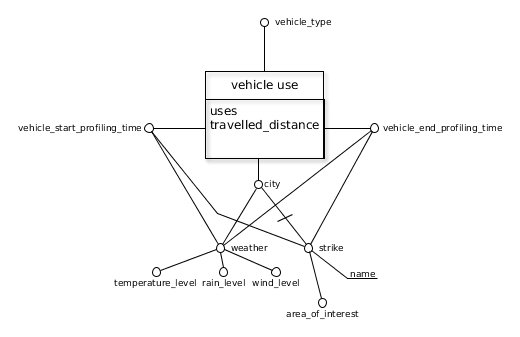
\includegraphics[width=\textwidth]{diagrams/dfm}                                                                                                                                   
\caption{DFM Vehicle use}                                                                                                                                            
\label{fig:dfm}                                                                                                                                                           
\end{figure}

Osservando il DFM si nota che gli attributi \textit{uses} e \textit{travelled\_distance} risultano
essere le misure scelte per il fatto in questione. Esse sono attributi di tipo numerico e
rappresentano rispettivamente il numero di utilizzi e la distanza percorsa mediante un determinato
veicolo.
Un'istanza di fatto è identificata dalla seguenti dimensioni:
\begin{itemize}
\item \textit{start\_profiling} e \textit{end\_profiling:} dimensioni di tipo data relative
rispettivamente all'istante di inizio e di fine di una finestra di profilazione; come è possibile
notare essi condividono la gerarchia che parte dall'attributo date e comprende tutti gli 
attributi discendenti quali \textit{day}, \textit{month}, \textit{year}, \textit{minute} e
\textit{hour};
\item \textit{vehicle\_type:} dimensione di tipo stirnga che permette la selezione tra diversi
tipi di veicoli all'interno di una finestra di profilazione;
\item \textit{city:} dimensione di tipo stringa caratterizzata dall'attributo descritto di tipo
stringa \textit{name}.
\end{itemize}

\section{Progettazione Logica e Fisica}
In questa Sezione viene descritto il processo di trasformazione del DFM, descritto al paragrafo precedente, in modello logico. 
Innanzitutto va specificato che è stata applicata la tecnica ROLAP (Relational On-Line Analytical Processing) che prevede l’utilizzo di un
modello relazionale per la rappresentazione dei dati multidimensionali.

\chapter{Analisi Sorgenti Dati}

\section{Helbiz}

Helbiz non mette a disposizione alcuna API pubblica per l'integrazione con
i servizi offerti né rilascia open data relativi agli utilizzi dei propri
veicoli. L'unico modo per un utente di interagire con un monopattino è mediante
l'applicazione mobile.

WoBike è un progetto presente su GitHub che raccoglie grazie al contributo
di alcuni sviluppatori la documentazione alle API dei principali 
provider di servizi di mobility sharing di tutto il mondo.
Tra le varie documentazioni presenti vi è il servizio di API REST
utilizzato dall'applicazione mobile di Helbiz, ottenuto per reverse
engineering dell'applicazione Android. A seguito di analisi e di relativo
utilizzo del servizio è emerso che lo stesso è stato oggetto di aggiornamento
nel tempo e che alcune richieste, una su tutte quella di autenticazione,
è cambiata per contenuto dei parametri inviati.
Si è reso pertanto necessario, da parte di chi scrive, procedere al reverse
engineering dell'applicazione Android. Tale operazione ha permesso di
identificare la variazione intervenuta e di procedere con successo
all'utilizzo del servizio in questione. Inoltre, allo scopo di facilitare
gli altri utenti interessati a tale servizio, sono state integrate nella
documentazione già presente, le variazioni rilevate alla richiesta di
autenticazione.

Un utente che decide di noleggiar per la prima volta un monopattino
deve nell'ordine:
\begin{itemize}
\item scaricare sul proprio smartphone o tablet l'applicazione ufficiale
disponibile su Play Store o App Store;
\item registrarsi al servizio attraverso l'applicazione;
\item abilitare la geolocalizzazione e abilitare l'applicazione ad accedere
alla propria posizione;
\item una volta geolocalizzato, scegliere un monopattino, dirigersi verso
il monopattino scelto ed inquadrarne il QR Code;
\item impostare il metodo di pagamento desiderato;
\item attendere lo sblocco del mezzo prima di poterlo utilizzare.
\end{itemize}
L'interazione con il monopattino necessita di una connessione dati, di
un dispositivo di geolocalizzazione, dell'accesso ad una fotocamera
per la scansione del QR Code.

\subsection{API REST}

Di seguito procediamo alla documentazione delle due richieste utilizzate,
tralasciando la richiesta per autenticazione ed altre richieste non
utili al progetto.

Ognuna delle successive richieste deve essere provvista dei seguenti
parametri nello header: \\

\begin{table}[h]
\centering
\begin{tabular}{|l|l|}
\hline
\rowcolor[HTML]{3166FF} 
{\color[HTML]{FFFFFF} \textbf{Chiave}} & {\color[HTML]{FFFFFF} \textbf{Valore}} \\ \hline
X-Requested-With                       & XMLHttpRequest                         \\ \hline
User-Agent                             & Helbiz (com.helbiz.android)            \\ \hline
Content-Type                           & application/json                       \\ \hline
X-access-token                         & Risultato richiesta di autenticazione  \\ \hline
\end{tabular}
\end{table}

\noindent~Ogni risposta fornita dal servizio qui descritto restituisce dei
dati in formato JSON.

\subsubsection{API Region}

\textbf{Method:} \texttt{GET} \\
\textbf{Url:} \texttt{https://api.helbiz.com/prod/regions} \\

\noindent\textbf{Descrizione:} la richiesta ritorna tutte le regioni corrispondenti
a città presso le quali Helbiz opera.
Relativamente alla singola region, gli attributi utilizzati all'interno del
progetto sono:
\begin{itemize}
\item name: nome della region in oggetto;
\item bounds: lista di coppie
\end{itemize}
coordinate cartesiane entra le quali è definita l'area della regione in
questione.
A seguito di analisi è risultato che i valori riportati per gli attributi
\emph{startTime} e \emph{endTime}, così come il valore dell'attributo live non sono
indicativi del periodi di attività o del funzionamento del servizio
nell'area in oggetto.
Il seguente listato contiene parte delle informazioni ritornate per
la città di Torino, ove presenti i puntini di sospensione va intesa
la presenza di altri dati per brevità non riportati.

\begin{figure}[H]
\centering
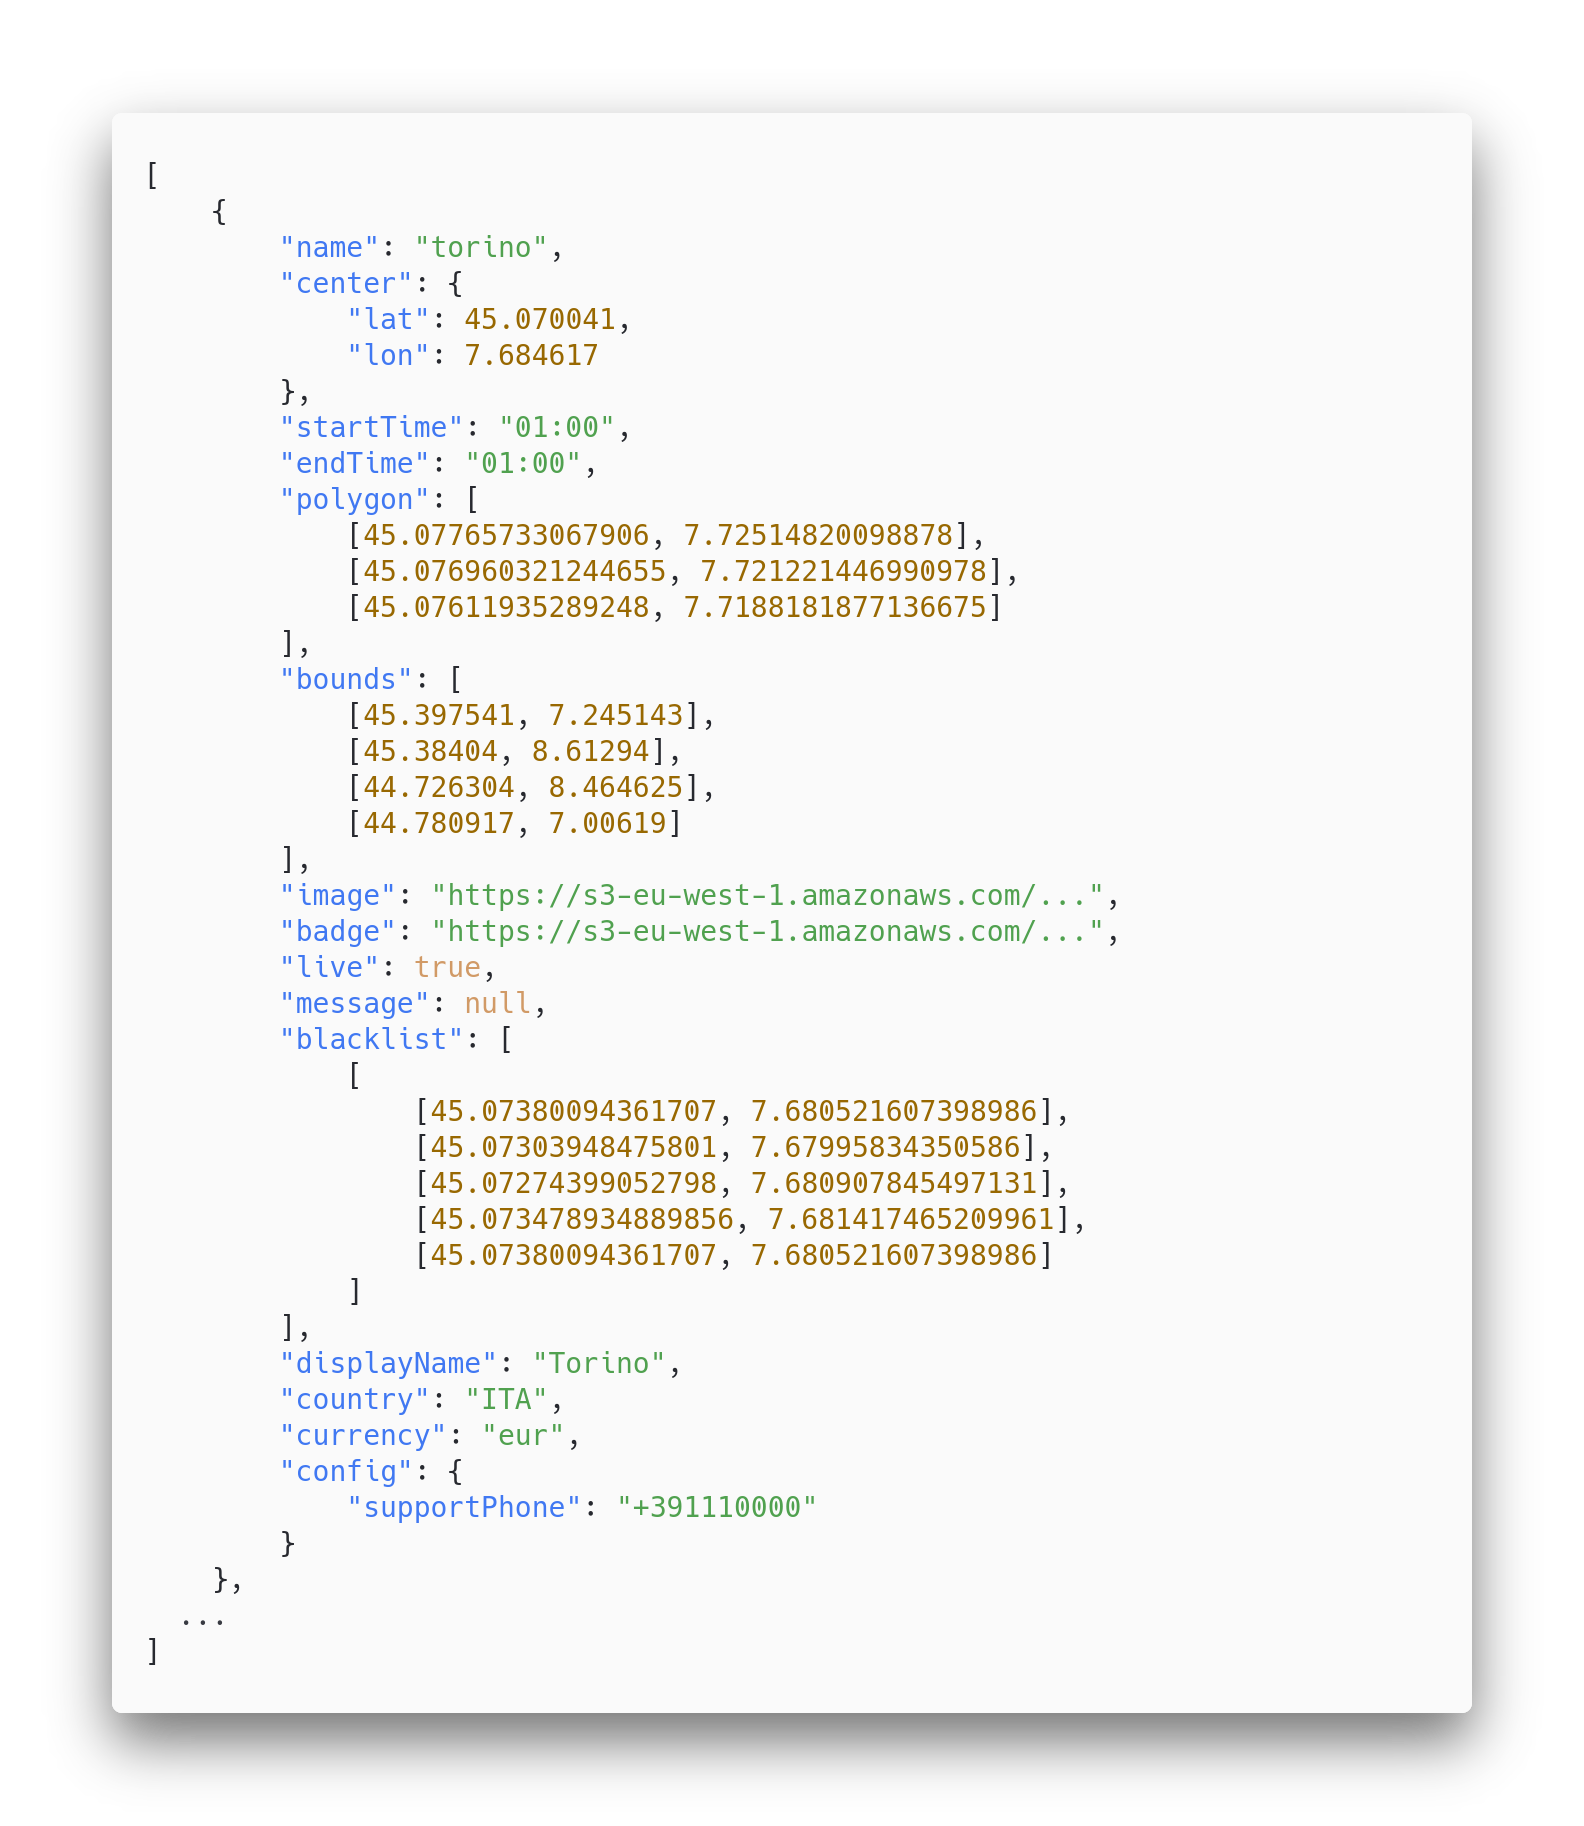
\includegraphics[width=\textwidth]{regionjson.png}
\caption*{Esempio di risposta API regions}
\label{fig:footprint}
\end{figure}


%\begin{minipage}[]{\linewidth}
%\inputminted[bgcolor=white]{json}{region.json}
%\end{minipage}

\subsubsection{API Vehicles}

\textbf{Method:} \texttt{GET} \\
\textbf{Url:} \texttt{https://api.helbiz.com/prod/vehicles?northWest=...\&southEast=...} \\

\begin{table}[h]
\centering
\resizebox{\textwidth}{!}{%
\begin{tabular}{|l|l|l|}
\hline
\rowcolor[HTML]{3166FF} 
{\color[HTML]{FFFFFF} \textbf{Parametro}} & {\color[HTML]{FFFFFF} \textbf{Esempio}} & {\color[HTML]{FFFFFF} \textbf{Descrizione}}                           \\ \hline
northWest                                 & 45,397541,7,245143                      & Coordinate geografiche dell'estremo Nord Ovest dell'area di interesse \\ \hline
southEast                                 & 44,726304,8,464625                      & Coordinate geografiche dell'estremo Sud Est dell'area di interesse    \\ \hline
\end{tabular}%
}
\end{table}

\noindent\textbf{Descrizione:} la richiesta ritorna i veicoli contenuti nell'area di interesse 
corrispondente al rettangolo avente per estremo superiore sinistro il punto specificato dal
parametro northWest e per estremo inferiore destro il punto specificato dal parametro southEast.
Relativamente al singolo veicolo, le informazioni utilizzate ai fini del progetto sono:
\begin{itemize}
\item id: identificatore del veicolo in formato di stringa alfanumerica (esedecimale);
\item lat: latitudine, numero provvisto di parte decimale di lunghezza variabile 
\item lon: longitudine, numero provvisto di parte decimale di lunghezza variabile
\item batteryLevelInMiles: autonomia in miglia della batteria, numero decimale 
\item range: valore risultante dal prodotto tra batteryLevelInMiles e 1000
\item geofence: nome della region di appartenenza
\end{itemize}
Il seguente listato contiene due veicoli di esempio ritornati interrogando il servizio
con le coordinate indicate nella precedente tabella e facenti riferimento alla \emph{region}
che copre la città di Torino.

%\inputminted[bgcolor=lightgray]{json}{vehicles.json}
\begin{figure}[H]
\centering
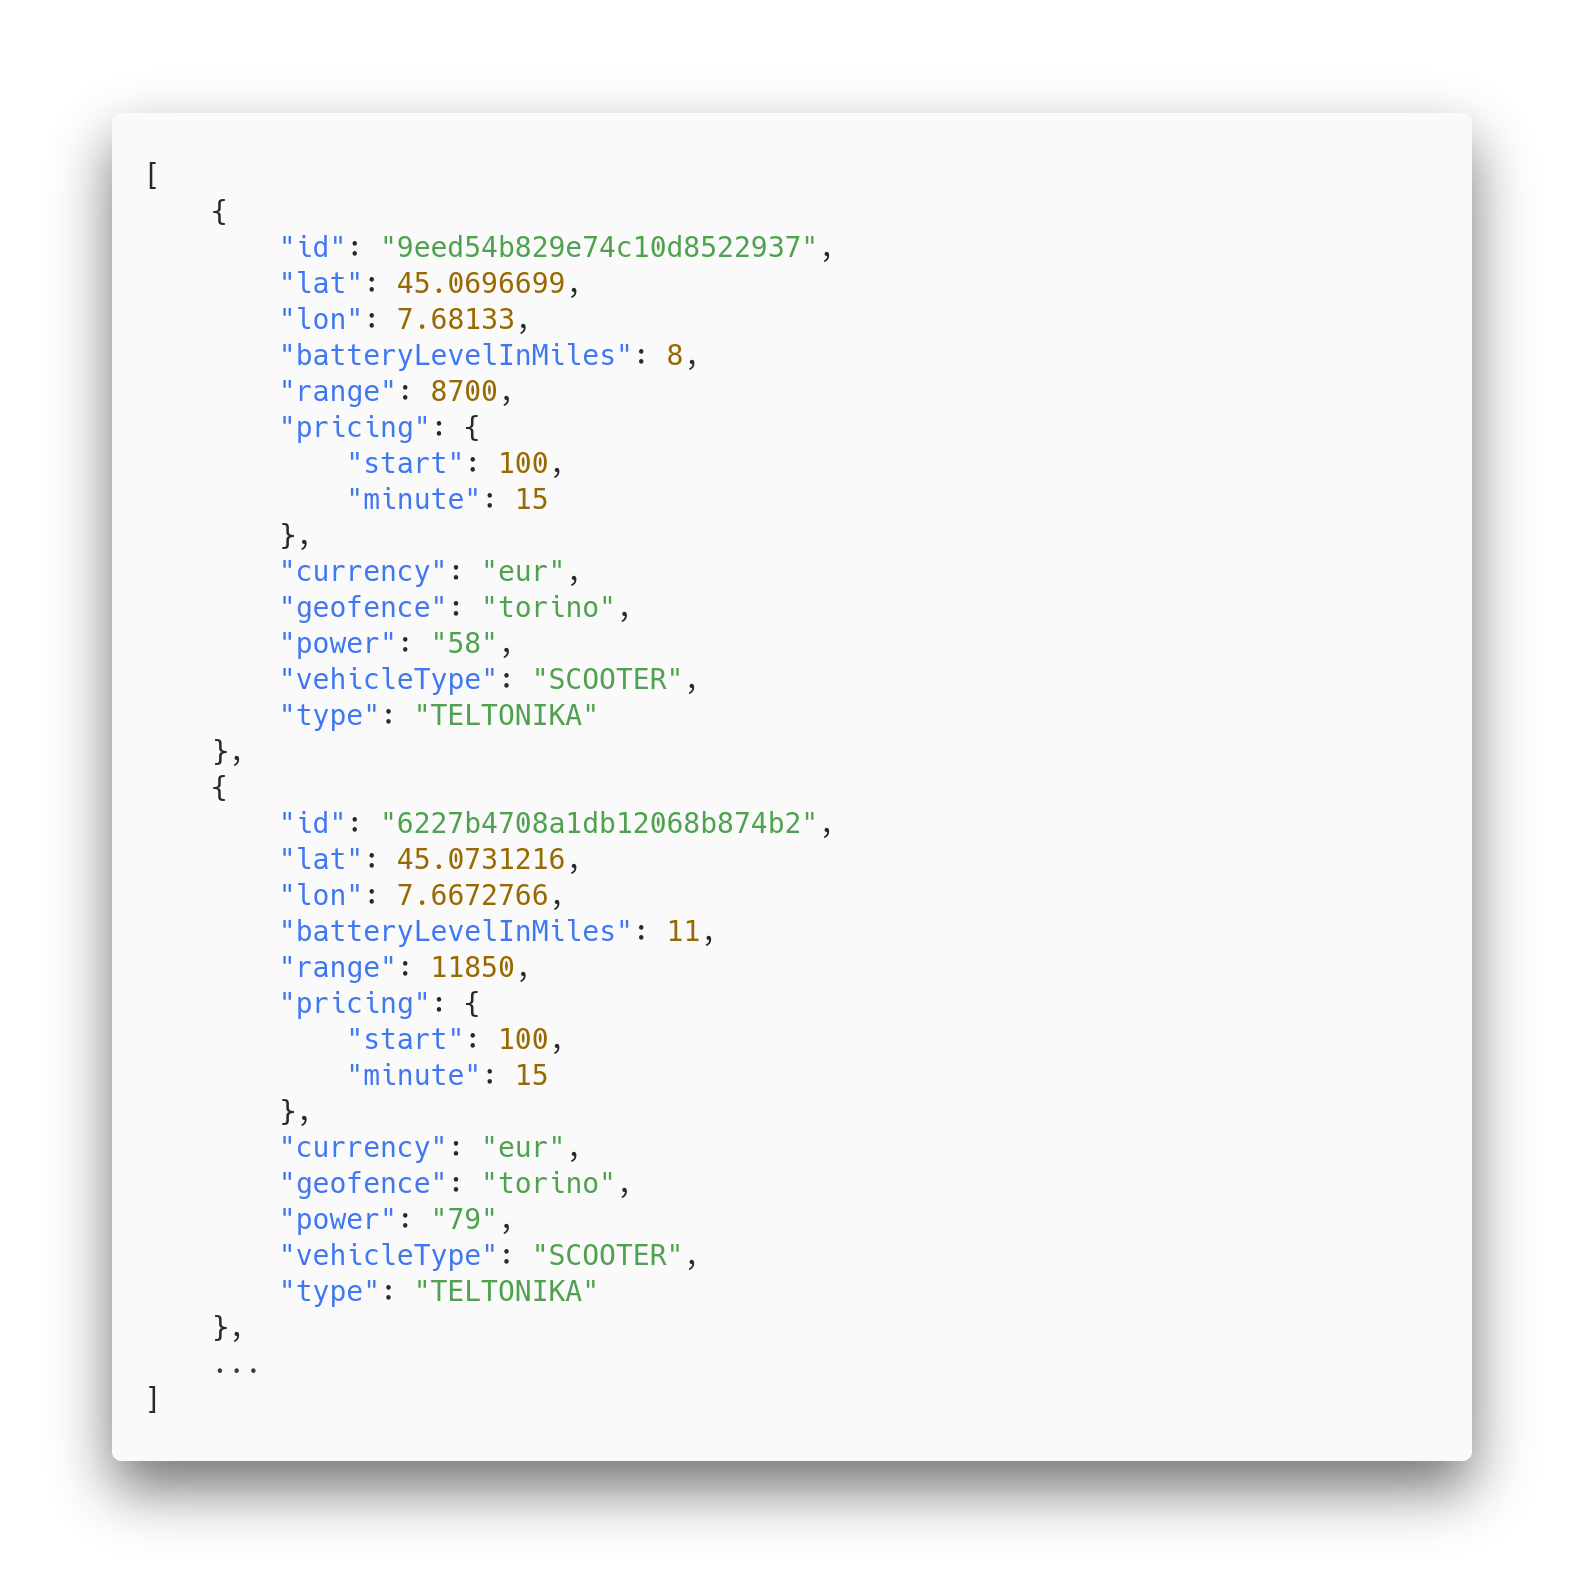
\includegraphics[width=\textwidth]{vehiclesjson.png}
\caption{vehicles.json}
\label{fig:vehiclesjson}
\end{figure}

\subsection{Progettazione concettuale}

A partire dalla API precedentemente descritta è stato scritto un applicativo Java,di cui
verrà fatta descrizione nel seguito, che partendo da una Region e da un intervallo in
minuti interroga ad intervalli regolari il servizio esposto da Helbiz per ottenere le
informazioni sui veicoli presenti in una delimitata area geografica.
In figura~\ref{fig:vehicle_profiling_er} è mostrato lo schema ER che modella le informazioni
relative alle profilazioni. Nella progettazione è stato assunto che ogni istanza
dell'entità Profiling sia univocamente identificata dall'attributo query\_time e
dall'attributo id dell'entità Vehicle.

\begin{figure}[H]                                                                                                                                                            
\centering                                                                                                                                                                   
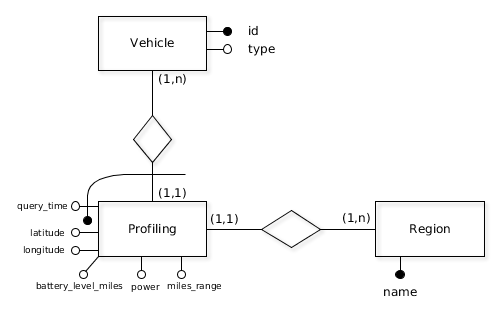
\includegraphics[width=\textwidth]{diagrams/vehicle_profiling_er}                                                                                                                                   
\caption{Diagramma ER Vehicle-Profiling-Region}                                                                                                                                            
\label{fig:vehicle_profiling_er}                                                                                                                                                           
\end{figure}

\subsection{Progettazione logica}

Risultato della progettazione logica sono le seguenti due relazioni:
\begin{itemize}
\item \textit{Vehicles:} contenente tutti dati relativi alla profilazione di un veicolo
appartenente ad una determinata regione in un dato istante di tempo; è presente un
vincolo di integrità referenziale per l'attributo \textit{region\_id} rispetto
all'attributo \textit{id} della relazione \textit{Regions};
\item \textit{Regions:} contenente i nomi delle regioni per le quali esistono delle
profilazioni all'interno della relazione \textit{Vehicles}.
\end{itemize}
In figura~\ref{fig:vehicles_logic_physic} è mostrato lo schema logico ottenuto mediante
l'applicativo MySQL Workbench.

Considerata a regime una differenza importante tra le due tabelle per numero di record
memorizzati, è stato valutata sconveniente l'aggiunta delle chiavi della tabella
\textit{Vehicles} alla tabella \textit{Cities} con conseguente aggiunta di ridondanza.
Ciò ha portato a trasformare la relazione uno a molto espressa nel precedente diagramma
ER in una relazione uno a uno. La stessa considerazione ha portato ad aggiungere
l'attributo \textit{type} dell'entità \textit{Vehicle} del precedente schema ER alla
tabella \textit{Vehicles} dello schema logico.

\begin{figure}[H]                                                                                                                                                            
\centering                                                                                                                                                                   
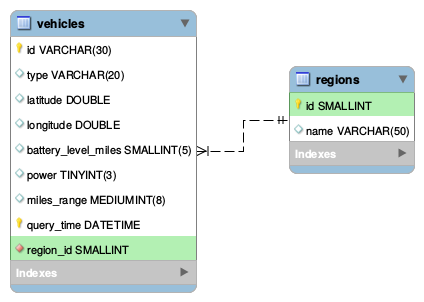
\includegraphics[width=\textwidth]{diagrams/vehicles_logic}                                                                                                                                   
\caption{Schema logico Vehicles}                                                                                                                                            
\label{fig:vehicles_logic_physic}                                                                                                                                                           
\end{figure}

\subsection{Note di utilizzo}

L'applicativo Java scritto per interrogare il servizio descritto sopra è stato attivo h24
per un periodo di un mese nell'interrogazione ad intervalli regolari di 5 minuti dei dati
della region relativa alla città di Torino.

\section{Torino Meteo}

\subsection{API REST}

\subsection{Progettazione concettuale}

In figura~\ref{fig:weather_detection_er} è mostrato lo schema ER per la sorgente in oggetto.
L'entità \textit{Weather sensor} è univocamente identificata dagli attributi id e detection\_time.

\begin{figure}[H]                                                                                                                                                            
\centering                                                                                                                                                                   
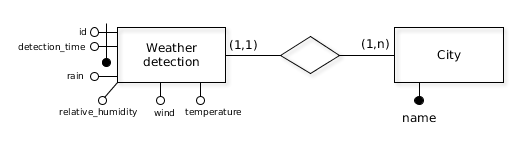
\includegraphics[width=\textwidth]{diagrams/weather_detection_er}                                                                                                                                   
\caption{Diagramma ER Weather sensor-City}                                                                                                                                            
\label{fig:weather_detection_er}                                                                                                                                                           
\end{figure}

\subsection{Progettazione logica}

Si è scelto di creare le seguenti due relazioni:
\begin{itemize}
\item \textit{Weather dectection:} contenente tutti i dati ottenuti interrogando un sensore;
l'attributo è stato posto un vincolo di integrità referenziale sull'attributo
\textit{city\_id} verso la relazione \textit{Cities};
\item \textit{Cities:} contenente i nomi delle città per le quali è presente almeno una
rilevazione nella relazione \textit{Weather detection}.
\end{itemize}
Lo schema logico prodotto è mostrato in figura~\ref{fig:weather_detection_logic}.
La relazione uno a molti tra l'entità \textit{Weather\_sensor} dello schema concettuale e
l'entità \textit{City} è stata trasformata in una relazione uno a uno in quanto, considerato 
a regime il numero di sensori di molto superiore al numero di città osservate, l'aggiunta di
due attributi alla relazione \textit{Cities} atti ad identificare un sensore in essa presente,
avrebbe comportato la presenza di ridondanza nei dati memorizzati.

\begin{figure}[H]                                                                                                                                                            
\centering                                                                                                                                                                   
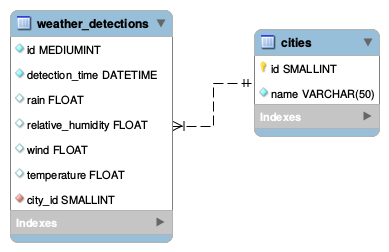
\includegraphics{diagrams/weather_detection_logic}                                                                                                                                   
\caption{Schema logico Weather detections}                                                                                                                                            
\label{fig:weather_detection_logic}                                                                                                                                                           
\end{figure}

\section{Scioperi}

\subsection{API REST}

\subsection{Progettazione concettuale}

In figura~\ref{fig:strikes_er} è presente il diagramma entità relazione per i dati
ottenuti dall'API descritta al punto precedente.
Le istanze dell'entità \textit{Strike} sono identificate univocamente dalla chiave composta
dagli attributi \textit{start\_time}, \textit{end\_time}, \textit{name} e \textit{City}.

\begin{figure}                                                                                                                                                            
\centering                                                                                                                                                                   
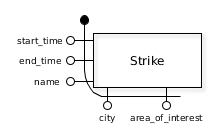
\includegraphics{diagrams/strikes_er}                                                                                                                                   
\caption{Diagramma ER Strike-City}                                                                                                                                            
\label{fig:strikes_er}                                                                                                                                                           
\end{figure}

\subsection{Progettazione logica}

Lo schema logico è mostrato in figura~\ref{fig:strikes_logic}.
Presupponendo il numero di scioperi di molto inferiore rispetto al numero di profilazioni
ottenute con le precedenti due sorgenti dati, è stata definita una sola relazione
\textit{Strikes} avente gli stessi attributi dell'entità \textit{Strike} del precedente 
schema ER.

\begin{figure}                                                                                                                                                            
\centering                                                                                                                                                                   
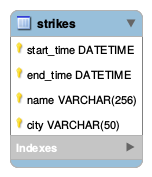
\includegraphics{diagrams/strikes_logic}                                                                                                                                   
\caption{Schema logico Strikes}                                                                                                                                            
\label{fig:strikes_logic}                                                                                                                                                           
\end{figure}

\chapter{Riconciliazione sorgenti}

Nel seguito verranno documentati i passi intrapresi nella progettazione
del modello riconciliato o Operational Data Store partendo dalle sorgenti
operazionali descritte nel capitolo precedente.

\section{Ispezione e normalizzazione}

\subsection{Helbiz}

Il livello di granularità delle profilazioni della sorgente Helbiz è
risultato essere troppo basso rispetto alle interrogazioni a cui il data
warehouse si prefigge di rispondere. Inoltre attributi come
\textit{latitude}, \textit{longitude}, \textit{battery\_level\_miles},
\textit{power} e \textit{miles\_range} non si prestano, in quanto valori
numerici continui, ad essere utilizzati all'interno del costrutto di
selezione di una interrogazione OLAP per il dominio applicativo
scelto. Infine, gli attributi \textit{battery\_level\_miles} e
\textit{miles} risultano essere ridondanti.

Partendo dallo schema ER mostrato in figura~\ref{fig:vehicle_profiling_er} è
stato ricavato lo schema concettuale di figura
\ref{fig:vehicle_interval_profiling_er}.

\begin{figure}[H]                                                                                                                                                            
\centering                                                                                                                                                                   
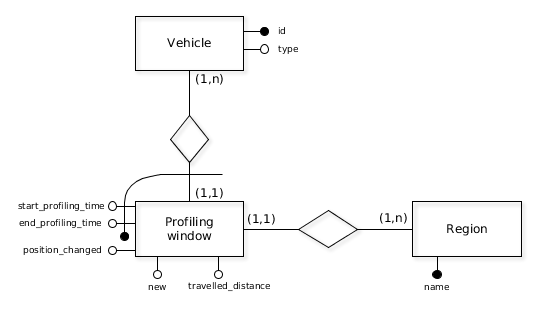
\includegraphics[width=\textwidth]{diagrams/vehicle_interval_profiling_er}                                                                                                                                   
\caption{Diagramma ER Vehicle-Profiling window-Region}                                                                                                                                            
\label{fig:vehicle_interval_profiling_er}                                                                                                                                                           
\end{figure}

Non essendo il nuovo schema una semplice ristrutturazione dello
schema logico di partenza ma un nuovo schema a se stante, l'entità
\textit{Profiling} è stata sostituita con l'entità \textit{Profiling
window}, le cui istanze si riferiscono ai dati profilati all'interno di
un delimitato intervallo di tempo per un determinato veicolo.
Nello specifico sono stati aggiunti i seguenti nuovi attributi:
\begin{itemize}
\item \textit{start\_profiling\_time:} istante di inizio della finestra
temporale;
\item \textit{end\_profiling\_time:} istante di fine della finestra temporale;
\item \textit{position\_changed:} attributo che indica se la posizione
del veicolo è variata durante l'intervallo in oggetto;
\item \textit{new:} attributo che indica se un veicolo non presente durante
all'istante di inizio della finestra temporale è stato invece censito
all'istante che delimita la fine della finestra temporale;
\item \textit{travelled\_distance:} attributo che contiene la distanza 
percorsa dal veicolo nella finestra temporale.
\end{itemize}

\noindent~L'attributo \textit{travelled\_distance} corrisponde alla distanza in linea
d'aria tra le coordinate cartesiane della profilazione effettuata all'istante
\textit{start\_profiling\_time} e quella effettuata all'istante
\textit{end\_profiling\_time}.
L'aggiunta dell'attributo \textit{new} è volta a gestire il caso in cui un
veicolo sia stato oggetto di utilizzo ininterrotto da parte di un utente per
un tempo superiore all'intervallo tra due successive profilazioni o il caso in
cui un veicolo sia stato intenzionalmente posizionato in un punto da un addetto
della manutenzione di Helbiz dopo essere stato ricaricato o allo scopo di
redistribuire la flotta di veicoli a disposizione all'interno della region.
L'attributo \textit{position\_changed} è stato aggiunto allo scopo di permettere
una veloce selezione delle istanze dell'entità in oggetto per le quali lo
spostamento memorizzato nell'attributo \textit{travelled\_distance} risulta essere
maggiore una certa soglia. Come sarà descritto nella parte dedicata alle attività di
ETL eseguite dalle sorgenti operazionali all'ODS, tale attributo permette di
escludere una serie di falsi positivi dati dalla presenza dei veicoli in ambienti
aperti, soggetti agli eventi atmosferici oltre che all'interazione con attori
che si trovano nelle immediate vicinanze.
Inoltre si ha che gli attributi \textit{start\_profiling\_time} e
\textit{end\_profiling\_time} insieme con l'attributo \textit{id} dell'entità
\textit{Vehicle}, identificano univocamente un'istanza dell'entità
\textit{Profiling window}.

Anche quest'ultimo schema risulta lontano dal poter essere integrato con le altre
sorgenti, aventi un livello di granularità temporale minimo di un'ora.
Inoltre gli attributi \textit{position\_changed} e \textit{new} non sono
sfruttabili in nessuna delle interrogazione derivate dal fatto definito.
Pertanto, partendo dallo schema concettuale di
figura~\ref{fig:vehicle_interval_profiling_er} si è giunti allo schema di figura
\ref{fig:vehicle_hour_profiling_er}.

\begin{figure}[H]                                                                                                                                                            
\centering                                                                                                                                                                   
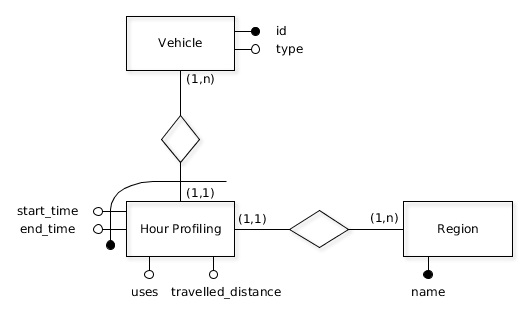
\includegraphics[width=\textwidth]{diagrams/vehicle_hour_profiling_er}                                                                                                                                   
\caption{Diagramma ER Vehicle-Profiling window-Region}                                                                                                                                            
\label{fig:vehicle_hour_profiling_er}                                                                                                                                                           
\end{figure}

Il processo di ristrutturazione ha consistito nella sostituzione dell'entità
\textit{Profiling window} con l'entità \textit{Hourly Profiling} avente i
seguenti nuovi attributi:
\begin{itemize}
\item \textit{start\_time:} istante d'inizio della finestra di profilazione;
\item \textit{end\_time:} istante di fine della finestra di profilazione;
\item \textit{uses:} attributo contenente il numero di utilizzi di un
veicolo all'interno della finestra di profilazione;
\item \textit{travelled\_distance:} attributo che contiene la distanza 
percorsa dal veicolo all'interno della finestra di profilazione.
\end{itemize}
Tale schema è pertanto da considerarsi quale schema concettuale definitivo per la
sorgente Helbiz e come uno degli schemi oggetto del successivo processo di
integrazione.

\subsection{Torinometeo}

Similmente a quanto fatto per Helbiz, anche per la sorgente Torinometeo è
stato necessario modificare lo schema concettuale presentato in figura
\ref{fig:weather_detection_er}. Le profilazioni acquisite dai sensori
sono relative ad un determinato istante di tempo e non ad una finestra temporale
come nel caso di Helbiz e riportano per gli attributi \textit{rain},
\textit{wind}, \textit{relative\_humidity} e \textit{temperature} valori numerici
continui che non si prestano ad essere utilizzati all'interno di interrogazioni
OLAP quali quelle definite. Inoltre, gli attributi \textit{id} e
\textit{relative\_humidity} non sono di interesse ai fini del progetto.
Lo schema derivato di figura \ref{fig:wheathre_hourly_profiling_er} contiene la
nuova entità \textit{Weather hourly profiling} caratterizzata dai seguenti attributi:
\begin{itemize}
\item \textit{start\_profiling\_time:} istante di inizio dell'intervallo orario in cui
si collocano le profilazioni rappresentate dall'entità in oggetto;
\item \textit{end\_profiling\_time:} ora di fine dell'intervallo orario in cui si
collocano le profilazioni rappresentate dall'entità in oggetto;
\item \textit{rain\_level:} attributo contenente il livello di intensità delle
precipitazioni, rilevato nell'intervallo orario;
\item \textit{wind\_level:} attributo contenente il livello di intensità del
vento, rilevato nell'intervallo orario;
\item \textit{temperature\_level:} attributo contenente il livello di intensità della
temperaturam rilevato nell'intervallo orario.
\end{itemize}

\begin{figure}[H]                                                                                                                                                            
\centering                                                                                                                                                                   
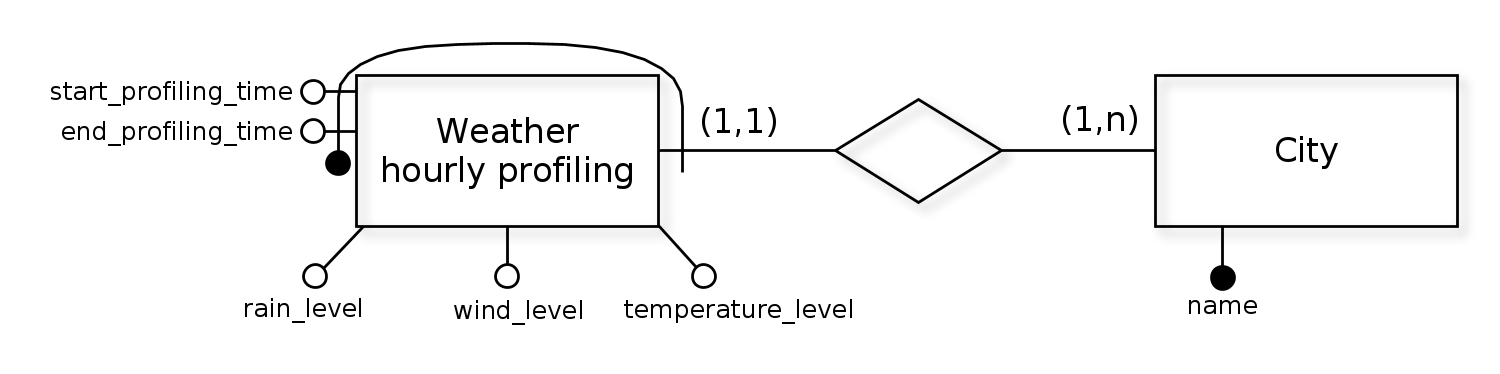
\includegraphics[width=\textwidth]{diagrams/wheathre_hourly_profiling_er}                                                                                                                                   
\caption{Diagramma ER Vehicle-Profiling window-Region}                                                                                                                                            
\label{fig:wheathre_hourly_profiling_er}                                                                                                                                                           
\end{figure}

Lo schema precedentemente descritto è da considerarsi quale schema concettuale definitivo
per la sorgente Torinometeo e come uno degli schemi partecipanti al successivo processo di
integrazione.

\subsection{Scioperi}

Per la sorgente Scioperi non è stato necessario procedere ad alcuna ristrutturazione dello
schema concettuale di figura~\ref{fig:strikes_er} che sarà pertanto insieme ai precedenti
oggetto della successivo processo di integrazione.

\section{Integrazione}

\subsection{Preintegrazione}

Essendo i dati relativi ad ogni sorgente operazionale considerata ottenuti
attraverso l'interrogazione di una API, solo un sottoinsieme tra entità,
relazioni e attributi rilevanti ai fini del progetto sono stati considerati
al momento della redazione dei precedenti schemi concettuali. Non è stato
quindi necessario escludere alcuna parte dei dati dall'integrazione. 

La semplicità dei diagrammi concettuali di ognuna delle tre sorgenti ha
permesso di utilizzare una strategia di integrazione n-aria single step.

\subsection{Comparazione e allineamento schemi}

\subsubsection{Conflitti sui nomi}

Si evidenzia tra lo schema concettuale della sorgente Helbiz e quello della
sorgente Torinometeo una sinonimia rispettivamente tra i nomi delle
relazioni \textit{Region} e \textit{City}. Le stesse vengono risolte nello
schema concettuale integrato utilizzando il nome \textit{City} per l'entità
in questione.

\subsubsection{Conflitti strutturali}
E' presente un conflitto strutturale relativo alla diversa rappresentazione 
dell'entità città, per le sorgenti Helbiz e Torinometeo come entità,
per la sorgente Scioperi come attributo dell'entità \textit{Strike}.
Si risolve tale conflitto adottando la rappresentazione come entità
come gestito negli schemi concettuali della altre due sorgenti.

\subsection{Fusione e ristrutturazione schemi}

Il risultato della sovrapposizione degli schemi e delle scelte intraprese nella
risoluzione dei conflitti ha portato allo schema di figura~\ref{fig:integrated_1_er}.

\begin{figure}[H]                                                                                                                                                            
\centering                                                                                                                                                                   
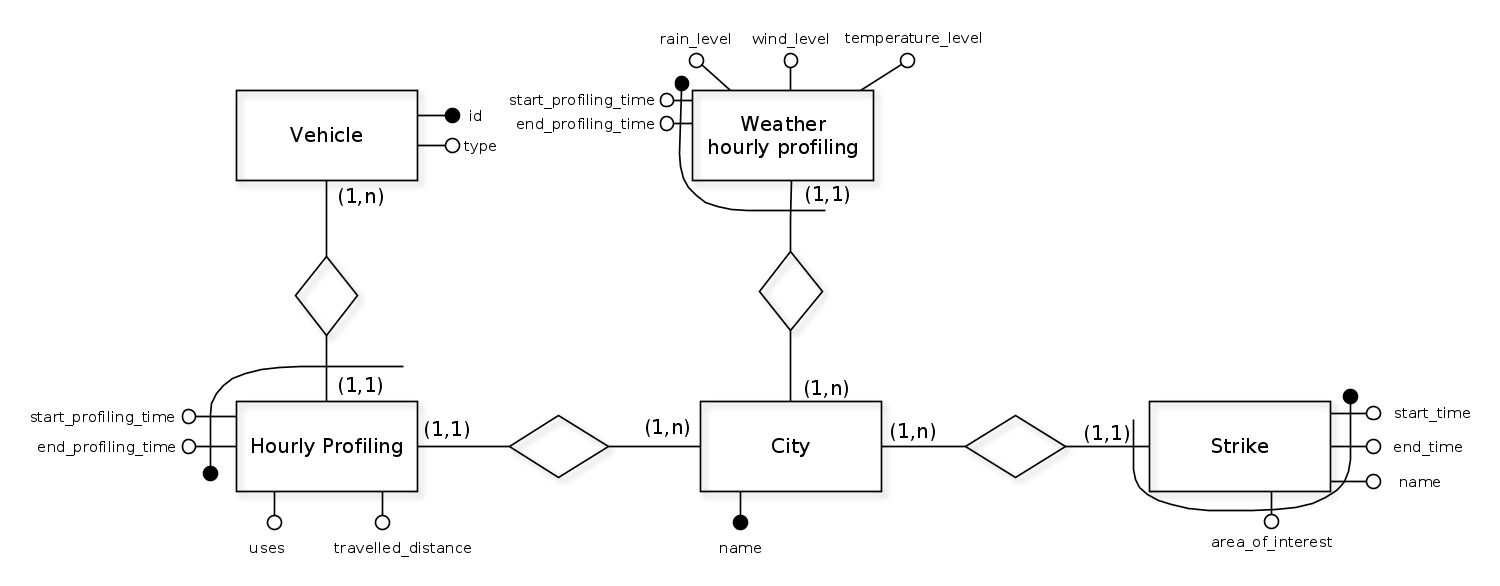
\includegraphics[width=\textwidth]{diagrams/integrated_1_er}                                                                                                                                   
\caption{Diagramma ER Vehicle-Profiling window-Region}                                                                                                                                            
\label{fig:integrated_1_er}                                                                                                                                                           
\end{figure}

In figura~\ref{fig:riconciliato_er} è mostrato lo schema logico dell'ODS.
Alla tabella \textit{cities} è stato aggiunta una chiave surrogata \textit{id}
verso la quale vi è un vincolo di integrità referenziale per ognuna delle tabelle
ad essa relazionate. Tale attributo è poi parte della chiave primaria per le
tabelle \textit{strikes} e \textit{weather\_hourly\_profilings}.

Diversamente da quanto fatto in fase di progettazione dello schema logico della
sorgente operazionale, si è scelto di rappresentare le entità \textit{vehicles}
e \textit{vehicles\_hourly\_profilings} con due relazioni eliminando la
ridondanza dell'attributo \textit{type}. 

Si noti inoltre la presenza dell'attributo \textit{insert\_time} per la
tabella \textit{cities}, verrà fatto riferimento allo stesso nelle due procedure
di ETL; nello specifico esso sarà popolato durante la fase di popolamento
dell'ODS e sarà letto nella fase di popolamento dei data mart.

\begin{figure}[H]                                                                                                                                                            
\centering                                                                                                                                                                   
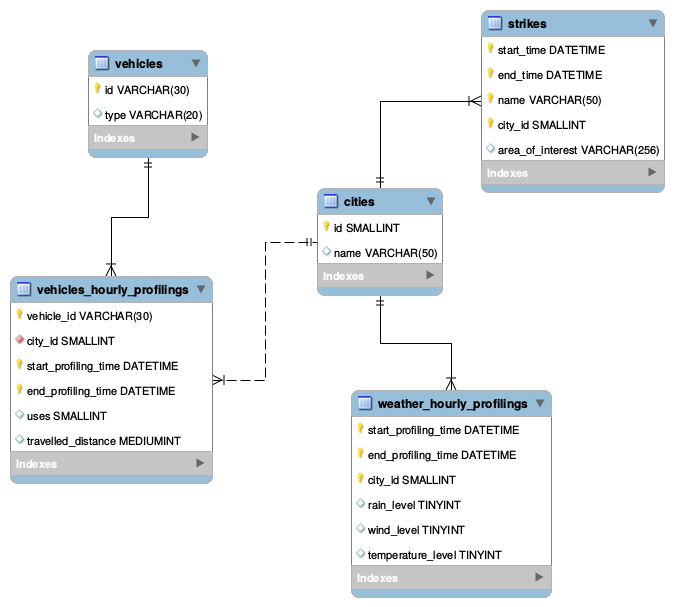
\includegraphics[width=\textwidth]{diagrams/riconciliato_er}                                                                                                                                   
\caption{Schema Riconciliato - Diagramma logico}                                                                                                                                            
\label{fig:riconciliato_er}                                                                                                                                                           
\end{figure}

\label{sec:etl_sorgenti_ODS}
\section{ETL da sorgenti operazionali a ODS}

\subsection{Helbiz}

\subsubsection{Estrazione}

La sorgente dati per sua natura di tipo transiente (i dati sono disponibili in
real-time e non sono disponibili dati storici) è stata trasformata in una
sorgente con dati periodici in quanto si è scelto di conservare i dati raccolti
mediante le API per un periodo di 6 mesi.

L'estrazione è di tipo \textit{incremental delayed}: un job di sistema è
schedulato al termine della giornata per invocare l'applicativo sviluppato in
modalità di estrazione il quale interroga la base dati, ottiene i dati delle
profilazioni delle ultime 24 ore e procedere al caricamento delle stesse
all'interno dell'ODS.

\subsubsection{Trasformazione}

Durante la procedura di estrazione viene interrogata la tabella
\textit{vehicles} dello schema di figura~\ref{fig:vehicles_logic_physic} al fine
di ottenere tutti gli istanti di profilazione intervenuti nelle ultime 24 ore
per una determinata region, ordinati in maniera crescente. Viene eseguita
a livello di codice Java la differenza tra coppie adiacenti di
\textit{query\_time} e vengono scartate le coppie per cui la differenza in
minuti non è compresa tra 3 e 10 minuti intervalli esclusi. Come anticipato
l'applicativo è stato impostato per acquisire dati dal servizio remoto ogni 5
minuti. Applicando tale operazione di filtraggio si ha la sicurezza di evitare
di processare profilazioni tra loro troppo vicine o troppo distanti, frutto in
qualche caso di errori dovuti alla momentanea incapacità di rispondere da parte
del servizio remoto. Per ogni coppia di istanti di misurazione viene effettuata
un'interrogazione al database della sorgente al fine di ottenere per ogni veicolo
della region di interesse una tupla ricavata dalla join della tabella
\textit{vehicles} con se stessa avendo cura di associare coppie di profilazioni
aventi stesso id, stessa città e diversa \textit{query\_time} preso dalla coppia
ottenuta. A questo punto, per ogni coppia vengono prese latitudine e longitudine,
convertite in radianti e viene calcolata la distanza in linea d'aria espressa in
metri mediante l'uso delle seguenti tre formule:

\begin{gather}
\varphi = \abs{\mathit{lon}_1 - \mathit{lon}_2}, \notag \\
\Delta = \arccos(\sin(\mathit{lat}_2) \cdot \sin(\mathit{lat}_1) + \cos{\mathit{lat}_2} \cdot \cos(\mathit{lat}_1) \cdot \cos(\varphi)), \notag \\
\mathit{d} = \Delta \cdot 6371000. \notag
\end{gather}

\noindent~Nello specifico, nell'ultima formula è utilizzato il raggio della
terra per calcolare la distanza tra i due punti. La distanza ottenuta è
confrontata con una soglia fissata a 100 metri. Se la distanza in linea d'aria
è superiore a tale valore, allora è possibile considerare che il veicolo in
questione sia stato utilizzato nell'intervallo considerato. Tale soglia serve
ad escludere errori nella segnalazione della posizione o spostamenti causati da
attori esterni con scopi diversi da quello di utilizzare il veicolo per spostarsi 
e pertanto non rilevanti allo scopo del progetto (\textit{e.g.} i veicoli possono essere spostati con un automezzo causa manutenzione o per operazioni stoccaggio). 
Quanto ottenuto da ogni coppia di veicoli è via via inserito in una query di INSERT che provvede ad inserire i risultati
nella tabella \textit{vehicles\_profilings} dell'ODS.
La colonna \textit{position\_changed} contiene un valore booleano sulla base
del precedente confronto eseguito sulla distanza in linea d'aria calcolata.
Al termine del processamento di tutte le coppie per un determinato intervallo,
viene eseguita un'altra query sulla tabella \textit{vehicles} della sorgente allo 
scopo di estrarre i veicoli rilevati nella misurazione più recente e non nella  
misurazione temporalmente precedente. In tal modo è possibile tenere conto dei
veicoli che in quanto utilizzati o disattivati non erano disponibili al momento 
della prima interrogazione ma lo sono diventati al momento della seconda. Per 
ognuno dei veicoli risultato di tale query è aggiunto un record alla tabella
\textit{vehicles\_profilings} avente valore nullo per le colonne 
\textit{position\_changed} e \textit{travelled\_distance} e valore
1 per la colonna booleana \textit{new}. La tabella \textit{vehicles\_profilings}
ha funzione di buffer per le successive operazioni di \textit{enrichment} e risiede
nell'ODS.

Al termine del processamento delle coppie di rilevazioni viene interrogata la tabella
appena riempita e vengono estratti tutti i record delle rilevazioni aventi come
\textit{start\_profiling\_time} un valore compreso nelle 24 ore precedenti.
Per ogni record estratto sono eseguite a livello di codice Java le seguenti
operazioni:
\begin{itemize}
\item l'attributo \textit{start\_profiling\_time} di tipo \java{DATETIME} viene
ricondotto all'inizio dell'ora ricavando così un'ora d'inizio;
\item viene verificata in una struttura dati di tipo \java{Map} allocata in
memoria la presenza di un valore passando come chiave l'attributo \textit{id}
del veicolo oggetto della profilazione; se presente, il valore ritornato consiste in un
oggetto di tipo \java{Map} che associa ad ogni ora di un giorno una mappa,
quest'ultima contenente le chiavi \textit{uses} e \textit{travelled\_distance}
ed i relativi valori numerici associati; in caso non esista un oggetto associato
all'ora passata come chiave, tale mappa viene creata e le viene associato
valore 0 per ognuno dei precedenti attributi;
\item se l'attributo \textit{position\_changed} è settato a 1 e la distanza
\textit{travelled\_distance} è inferiore a 3000 metri, l'algoritmo procede
ad incrementare la entry con chiave \textit{uses} e ad aggiungere la distanza
percorsa all'attributo \textit{travelled\_distance}; considerando che i veicoli
in esame hanno una velocità massima di 25\,km/h, e da ciò che la massima distanza
percorribile in un tempo di 5 minuti è di 2\,km, la cifra limite utilizzata nel
precedente confronto è stata ottenuta moltiplicando per 1,5 tale distanza;
\item se l'attributo \textit{new} è invece settato a 1, viene eseguito
un controllo tra le profilazioni aventi \textit{end\_profiling\_time} eguale
alla \textit{start\_profiling\_time} corrente e, nel caso in cui tale veicolo
risulti presente in tale finestra di profilazione antecedente a quella in oggetto
se ne calcola la distanza percorsa con l'utilizzo delle formule mostrate in
precedenza; nel caso in cui la distanza risulti realisticamente percorribile
nel corso di 10 minuti di tempo, allora si procede con le stesse modalità
del punto precedente all'incremento degli attributi \textit{uses} e
\textit{travelled\_distance}.
\end{itemize}
I dati contenuti nella mappa presente in memoria vengono inseriti nella
tabella \textit{vehicles\_hourly\_profilings}, appartenente anch'essa all'ODS
e risultato del precedente processo di integrazione.

Ogni region ha come attributo un nome sotto forma di stringa alfanumerica
minuscola. E' però necessario convertire tale stringa nel nome
della corrispondente città, valore utilizzato dalle altre due sorgenti
oggetto dell'integrazione. Entra quindi in gioco una procedura di
\textit{cleansing} che utilizzando una tabella di supporto, provvede a
modificar il valore dell'attributo \textit{city\_id} della tabella
\textit{vehciles\_profilings} con l'id della corrispondente città della
tabella \textit{cities} dell'ODS, il tutto mediante una query di UPDATE
la quale esegue una JOIN su di una tabella di traduzione appositamente
definita. Con tale operazione termina la procedura di trasformazione dei dati.

\subsubsection{Caricamento}

La procedura di caricamento è di tipo incrementale, consiste nella sola aggiunta di
nuovi record alla tabella e viene eseguita con cadenza giornaliera al termine della
procedura di trasformazione. Il tutto è svolto dall'applicativo Java sviluppato che
si occupa nell'ordine di:
\begin{itemize}
\item inserire nella tabella \textit{vehicles} i record relativi a veicoli non ancora
inseriti che sono stati oggetto di profilazioni durante la giornata precedente;
\item inserire nella tabella \textit{cities} i record relativi a nuove città oggetto
di profilazione durante la giornata precedente; ad ogni record inserito corrisponderà
un orario di inserimento memorizzato nell'attributo \textit{insert\_time} della stessa
tabella;
\item estrarre i dati dalla tabella \textit{cities} della sorgente e utilizzare la
tabella di traduzione al fine di verificare la presenza della versione tradotta della
stessa all'interno dell'ODS e in caso contrario procedere all'aggiunta;
\item estrarre dal database delle sorgente i record inseriti durante la precedente
giornata (per i quali l'attributo \textit{query\_time} si riferisce ad un istante che
si colloca nelle precedenti 24 ore) comprensivi dell'attributo \textit{name} della
tabella \textit{city};
\item procedere all'inserimento dei record ottenuti al punto precedente ottenendo
per ogni valore dell'attributo \textit{cities.name}, per mezzo del costrutto JOIN,
il \textit{city\_id} corrispondente della tabella \textit{cities} dell'ODS, al fine
di mantenere l'integrità referenziale.
\end{itemize}

\subsection{Torinometeo}

\subsubsection{Estrazione}

Si ha a che fare con una sorgente con dati periodici per la quale si è scelto di 
conservare dati per i successivi 6 mesi a partire dalla raccolta degli stessi.

L'estrazione è di tipo \textit{incremental delayed}: un job di sistema è
schedulato al termine della giornata per invocare l'applicativo sviluppato in
modalità di estrazione il quale interroga la base dati, ottiene i dati
memorizzati nelle ultime 24 ore e procedere al caricamento degli stessi
all'interno dell'ODS.

\subsubsection{Trasformazione}

Come anticipato, i dati raccolti nel database della sorgente sono relativi a
misurazioni realizzate dal sensore nell'istante in cui quest'ultimo viene
interrogato. Tali dati non si prestano ad essere associati alle rilevazioni
sull'utilizzo orario dei veicoli. Segue una procedura di enrichment la quale
provvede nell'ordine a:
\begin{itemize}
\item trasformare il valore di tipo \java{DATETIME} dell'attributo
\textit{query\_time} nell'ora esatta precedente più prossima (operazione
equivalente ad azzerare minuti e secondi);
\item eseguire la media delle somme degli attributi \textit{wind\_level},
\textit{temperature\_level} e \textit{rain\_level} di tutti i record per i
quali l'attributo \textit{query\_time} rappresenta lo stesso istante o un
istante più recente, distante meno di un'ora dalla data calcolata al punto
precedente;
\item confrontare per ognuno degli attributi calcolati la relativa tabella
dei livelli la quale associa un valore da 0 a 4 sulla base dell'appartenenza
o meno al range di valori associato al livello corrispondente; in tal modo si
rendono discreti i valori di tali attributi e quindi candidati ad essere 
oggetto di interrogazione;
\item creare un record da inserire nella tabella
\textit{weather\_hourly\_profilings} a partire dai dati ottenuti ai punti
precedenti; nello specifico, per l'attributo
\textit{start\_profiling\_time} viene presa la data calcolata al primo punto;
a tale data è sommata un'ora per ottenere il valore dell'attributo
\textit{end\_profiling\_time}; ad ognuno degli attributi relativi alle
condizioni atmosferiche è associato il livello ottenuto al punto precedente;
l'attributo \textit{city\_id} è invece ottenuto per mezzo di una JOIN tra il
nome della città estratta dalla base dati della sorgente e la tabella
\textit{cities} dell'ODS.
\end{itemize}
Tali passi sono ripetuti per ogni ora della precedente giornata.

Le operazioni precedenti, eseguite interamente attraverso l'esecuzione di query 
SQL, sono eseguite dall'applicativo Java scritto al termine della precedente
procedura di estrazione.

\subsubsection{Caricamento}

Il caricamento è di tipo incrementale e consiste nella sola aggiunta dei nuovi
record alla tabella \textit{weather\-hourly\_profilings} e avviene con cadenza
giornaliera al termine della precedente procedura di trasformazione.
L'applicativo Java preposto si occupa di:
\begin{itemize}
\item inserire nella tabella \textit{cities} i record relativi a nuove città oggetto
di profilazione durante la giornata precedente;
\item procedere all'inserimento dei record risultanti dalla precedente procedura di
trasformazione facendo in modo di inserire per l'attributo \textit{city\_id}
la corrispondente chiave della tabella \textit{cities} dell'ODS, al fine
di mantenere l'integrità referenziale.
\end{itemize}

\subsection{Scioperi}

\subsubsection{Estrazione}

Si ha a che fare con una sorgente con dati periodici per la quale si è scelto di 
conservare dati per i successivi 6 mesi a partire dalla raccolta degli stessi.

Come per le altre due sorgenti l'estrazione è di tipo
\textit{incremental\_delayed} ed è effettuato con le stesse modalità utilizzate
dalle precedenti.
E' invece presente una differenza sui dati
memorizzati che si riferiscono a scioperi avvenuti non meno di due giorni prima
della data corrente. Come anticipato al momento della descrizione della sorgente,
tali open data hanno anche funzionalità di forecasting ricomprendendo tra gli scioperi
anche quelli previsti nel futuro ed annunciati. Gli scioperi, compresi quelli in corso,
sono soggetti a modifiche ed annullamenti. Considerato che il dato sulla
presenza o meno di uno sciopero è da ritenersi attendibile solo al termine dello
sciopero stesso, si è scelto di inserire ad ogni aggiornamento della base dati
della sorgente i dati sui soli scioperi aventi data precedente di due giorni la
data corrente al fine di gestire anche il caso di scioperi della durata superiore 
ad un giorno.

Inoltre, al fine di ottimizzare il processo di estrazione, nell'interrogazione
vengono selezionati i record degli scioperi relativi alle sole città di interesse,
ovvero quelle presente nella base dati della sorgente Helbiz.

\subsubsection{Trasformazione}

Non è stata compiuta alcuna trasformazione sui i dati della sorgente Scioperi.

\subsubsection{Caricamento}

Nel caso in cui uno sciopero sia indetto a livello nazionale e sia quindi esteso
a tutte le città, esso riporterà come valore del campo \textit{city} la stringa 
"Tutte". Si è scelto di aggiungere un record dummy alla tabella \textit{cities}
avente come attributo \textit{name} la stringa suddetta.

Al termine della procedura di estrazione, per ogni record del database della
sorgente viene ottenuto mediante il costrutto JOIN il relativo id della tabella
\textit{cities}; questo è inserito come attributo \textit{city\_id} per la
nuova tabella.

\include{alimentazione}
\chapter{Interrogazione del data mart}
In questa sezione vengono definite le interrogazioni sui datamart che sono state effettuate.

Tutte le richieste fatte ai datamart vengono, di conseguenza, effettuate attraverso interroga-
zioni ad un DBMS Mysql.

\section{Visualizzazione settimanale}

\begin{figure}[H]                                                                                                                                                            
\centering                                                                                                                                                                   
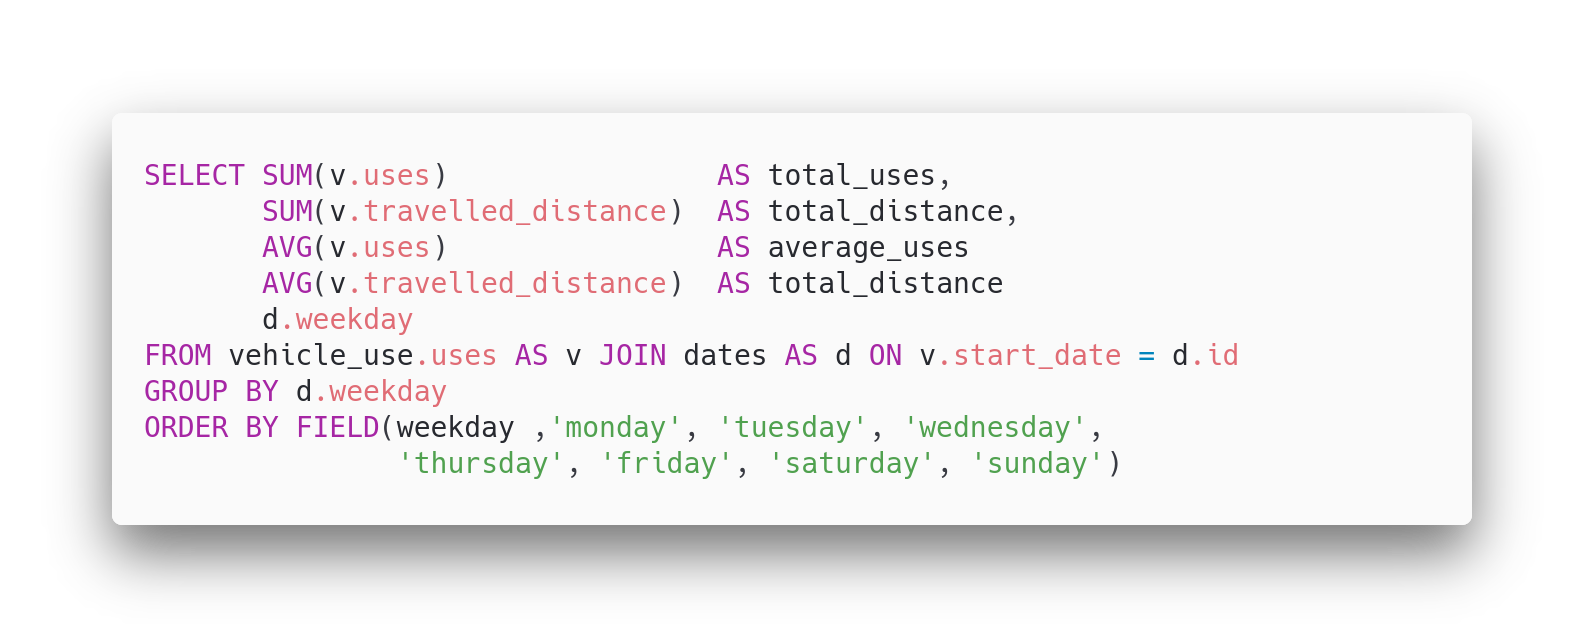
\includegraphics[width=\textwidth]{images/query1}                                                                                                                                   
\label{fig:query1}                                                                                                                                                           
\end{figure}

\iffalse
SELECT SUM(v.uses)                AS total_uses, 
	   SUM(v.travelled_distance)  AS total_distance, 
       AVG(v.uses)                AS average_uses
       AVG(v.travelled_distance)  AS total_distance
       d.weekday
FROM vehicle_use.uses AS v JOIN dates AS d ON v.start_date = d.id
GROUP BY d.weekday
ORDER BY FIELD(weekday ,'monday', 'tuesday', 'wednesday',
			   'thursday', 'friday', 'saturday', 'sunday')
\fi


\section{Utilizzo per livelli di pioggia mese per mese}
\begin{figure}[H]                                                                                                                                                            
\centering                                                                                                                                                                   
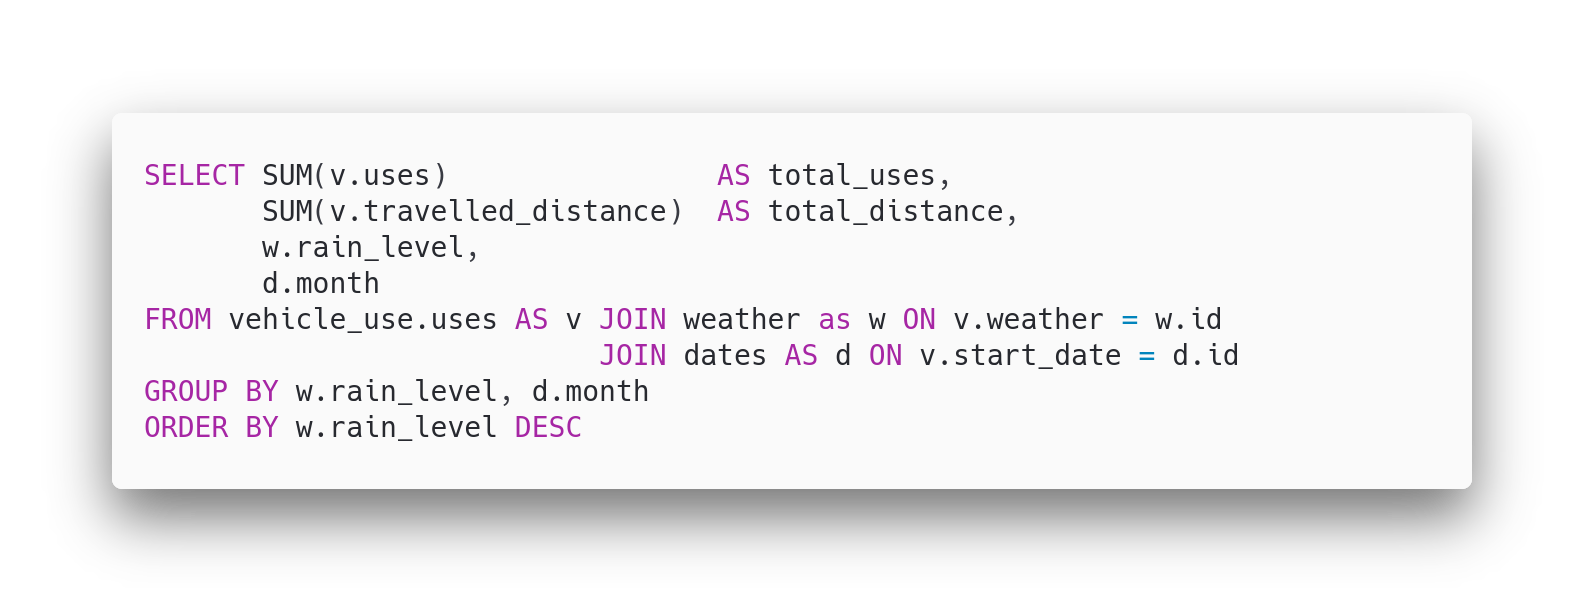
\includegraphics[width=\textwidth]{images/query2}                                                                                                                                   
\label{fig:query2}                                                                                                                                                           
\end{figure}
\iffalse
SELECT SUM(v.uses)                AS total_uses, 
	   SUM(v.travelled_distance)  AS total_distance,
       w.rain_level,
       d.month
FROM vehicle_use.uses AS v JOIN weather as w ON v.weather = w.id
                           JOIN dates AS d ON v.start_date = d.id
GROUP BY w.rain_level, d.month
ORDER BY w.rain_level DESC
\fi

\end{document}
